The ``fake rate'' method is used to estimate the background
from $\Wjets$ and QCD events, where at least one of the jets or a
constituent is misidentified as an isolated lepton.  This method
is described in detail in Refs.~\cite{fakeLeptonNote1} 
and~\cite{fakeLeptonNote2}. In brief, 
we define set of loosely selected lepton-like objects, referred to as the 
``fakeable object'' or ``denominator'' from here on, in a 
sample of events dominated by dijet production. 
The efficiency for these denominator objects to pass 
the full lepton selection critera is measured. 
This background efficiency, typically referred to as the ``fake rate'', 
is parameterized as a function of the $\pt$ and $\eta$ of the denominator 
object in order to capture any dependence on kinematic and geometric quantities. 
We will denote the fake rate symbollically by $\epsilon_{\mathrm{fake}}$.
These fake rates are, then, used as weights to extrapolate
the background yield from a sample of loose denominator objects to the sample
of fully selected leptons. The denominator definitions
used in the HCP 2012 analysis remain unchanged from those described in
Ref.~\cite{hcp2012Note}.

Real leptons can contribute to the dijet control region
through the production and subsequent leptonic decays of W and Z bosons.
To reduce the W contribution in the previous analysis, we 
required the $\met$ to be less than 20 GeV. To
reduce the Z contribution, we required
there to be no second lepton in the detector 
meeting the denominator requirement. In this analysis 
we tighten these requirements, and use simulation to estimate
and subtract the residual electroweak contamination.

To further reduce the contribution from W decays, we require $\mt$
below 15 GeV.  To estimate the residual contribution to the 
dijet control sample, we use W+jets simulation normalised to
the calculated luminosity for the prescaled triggers used to
acquire the control sample.  We apply an additional scale factor
to the W+jets simulation to take into account residual data-simulation
differences, derived by inverting the W+jets rejection requirements
to $\met>$30 GeV and $60<\mt<90$ GeV and requiring the full lepton selection.
The systematic uncertainty 
on the W+jets prediction is taken to be the magnitude of the difference 
of the scale factor from unity.  The scale factor is 
$0.81 \pm 0.19 \mathrm{(syst.)}$ and $1.06 \pm 0.06 \mathrm{(syst.)}$
in the muon and electron final states respectively. The agreement
between data and simulation after applying these scale factors 
is shown in Figure \ref{fig:wjets_ctl}.

\begin{figure}[!hbtp] 
\centering
\subfigure[]{
\centering
\label{subfig:el_wjets_ctl}
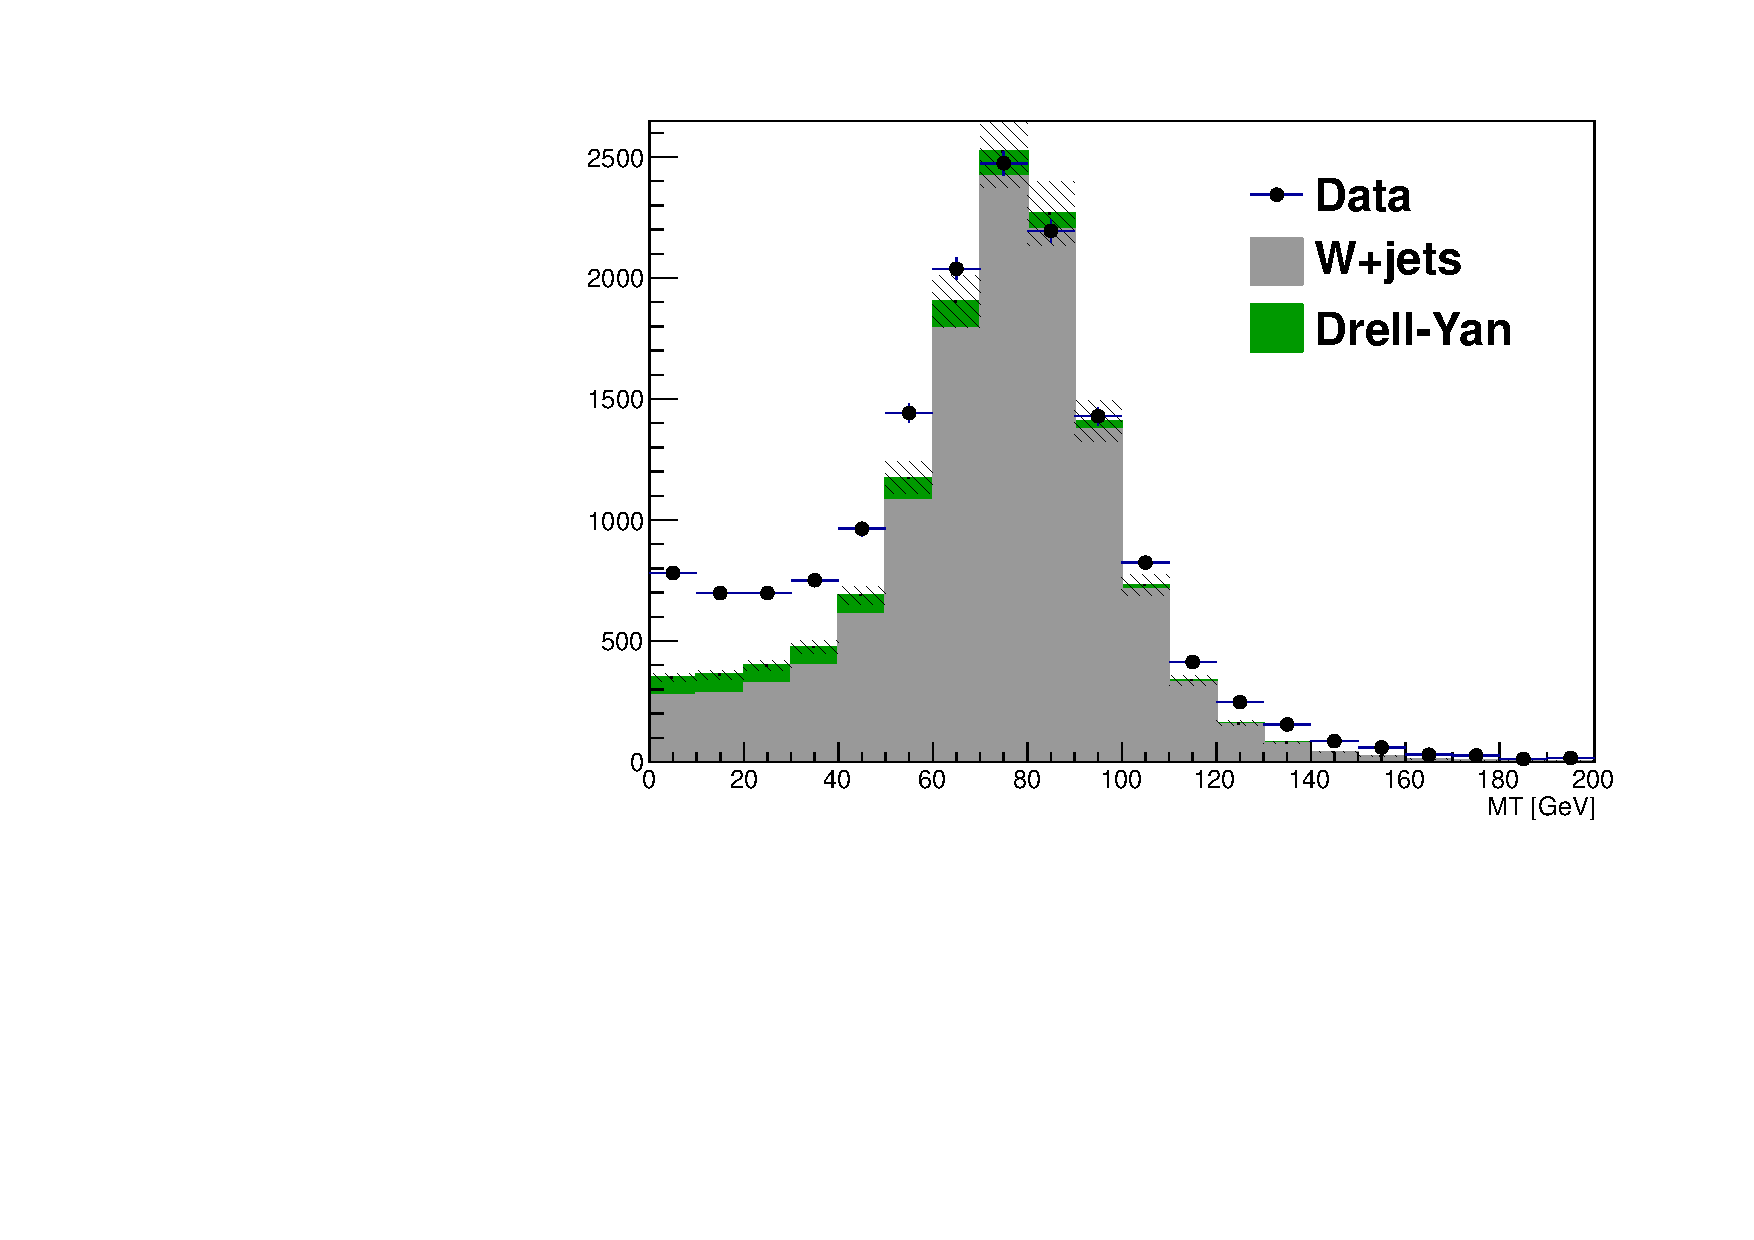
\includegraphics[width=.4\textwidth]{figures/ElectronFakeRate_V4_num_highPt_mt_met20mt15mll_Moriond.pdf}
}
\subfigure[]{
\centering
\label{subfig:mu_wjets_ctl}
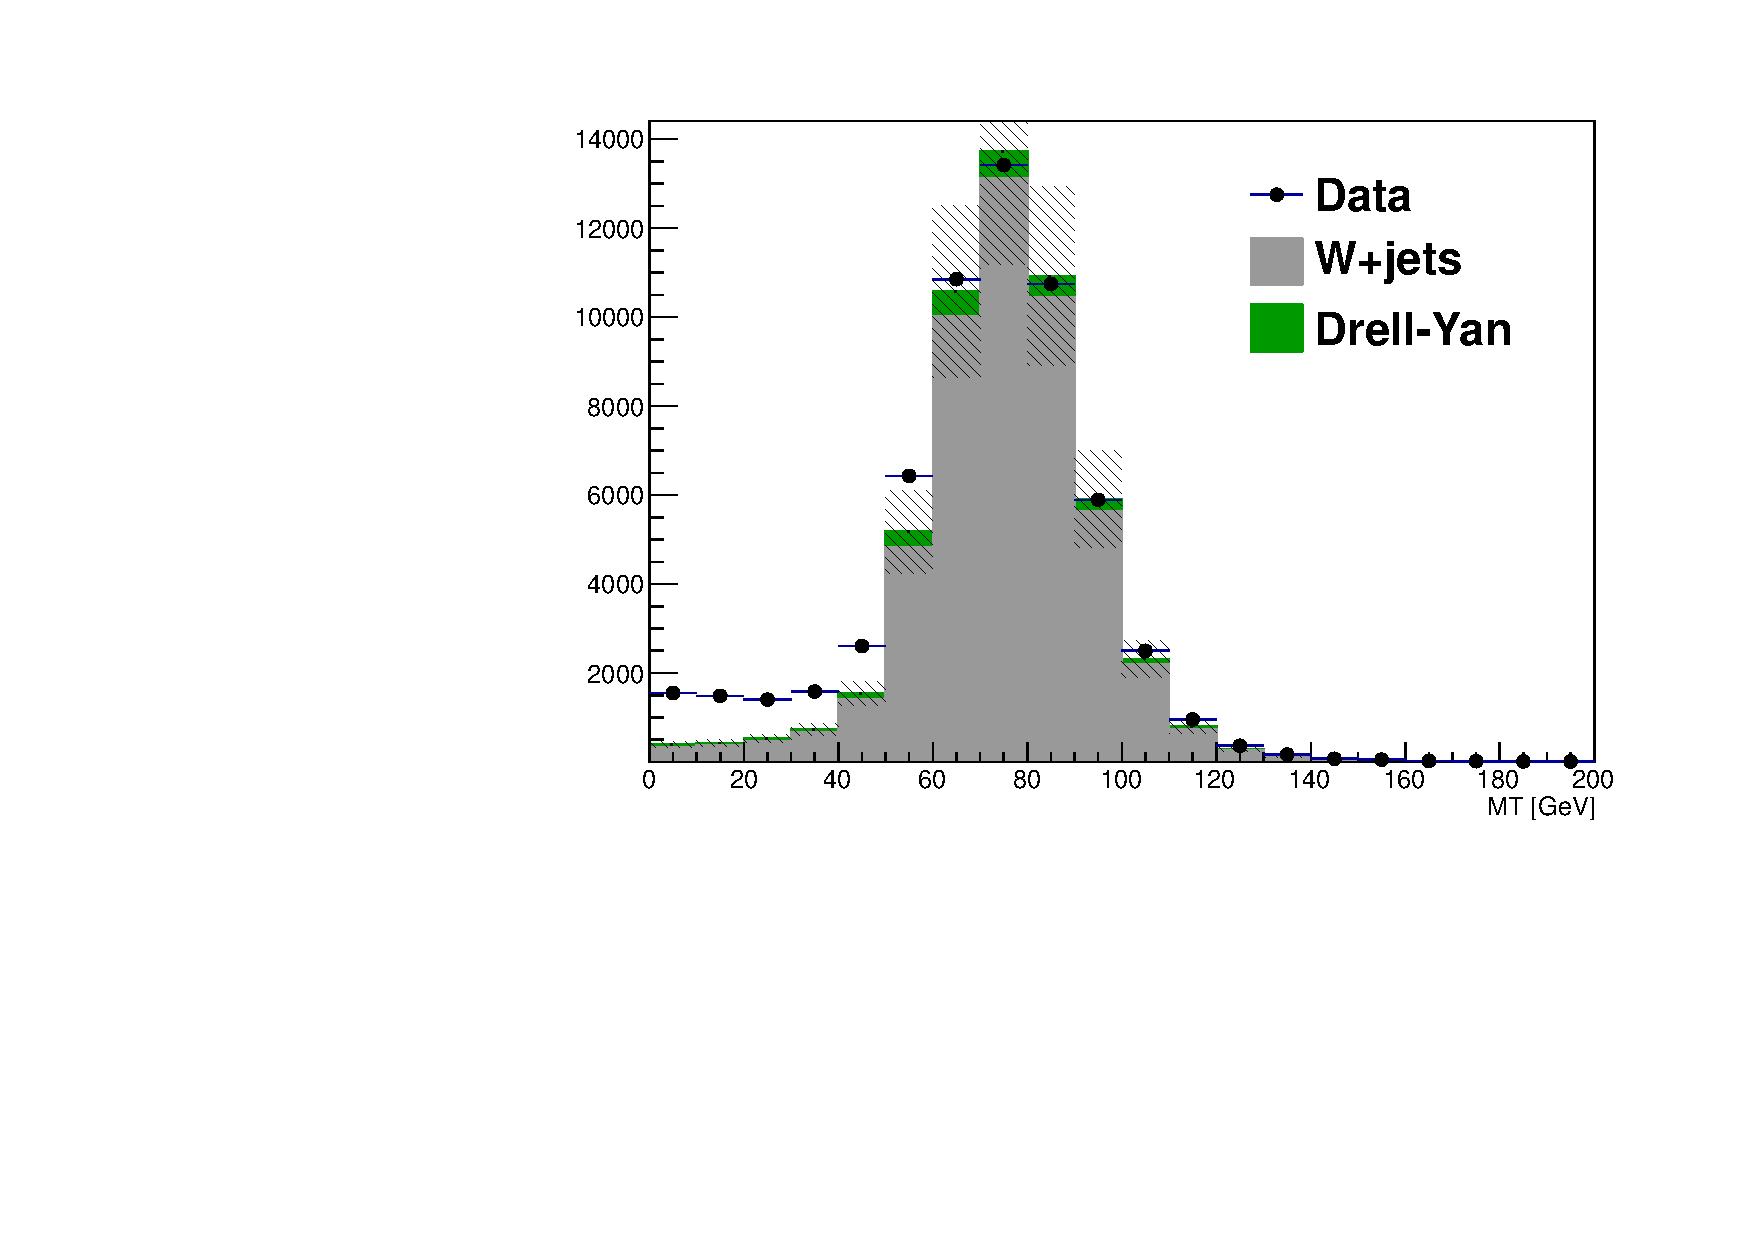
\includegraphics[width=.4\textwidth]{figures/MuonFakeRate_M2_num_highPt_mt_met20mt15mll_Moriond.pdf}
}\\
\caption{W+Jets control region in the fake rate derivation sample 
for muons (\ref{subfig:mu_wjets_ctl}) and electrons (\ref{subfig:el_wjets_ctl})
where FO passes the numerator and MET $>$ 30 GeV. 
The default jet pt threshold is applied, and the DY background is subtracted from simulation.}
\label{fig:wjets_ctl} 
\end{figure}

To further reduce the contibution from Z decays, we tighten
the second lepton veto to reject any event with a second
reconstructed electron or muon if the pair have opposite
sign and an invariant mass within 15 GeV of the Z boson mass.
We apply an additional scale factor to the Z simulation
to take into account residual data-simulation differences,
derived by inverting the invariant mass veto.  The Z scale 
factor is derived after the subtraction of residual QCD backgrounds
by using same sign events.  The values are $1.15 \pm 0.15 \mathrm{(syst.)}$
and $0.94 \pm 0.06 \mathrm{(syst.)}$ for the muon and electron
final states respectively.  The agreement between data and simulation
after applying these scale factors is shown in Figure \ref{fig:zjets_ctl}.

\begin{figure}[!hbtp]
\centering
\subfigure[]{
\centering
\label{subfig:el_zjets_ctl}
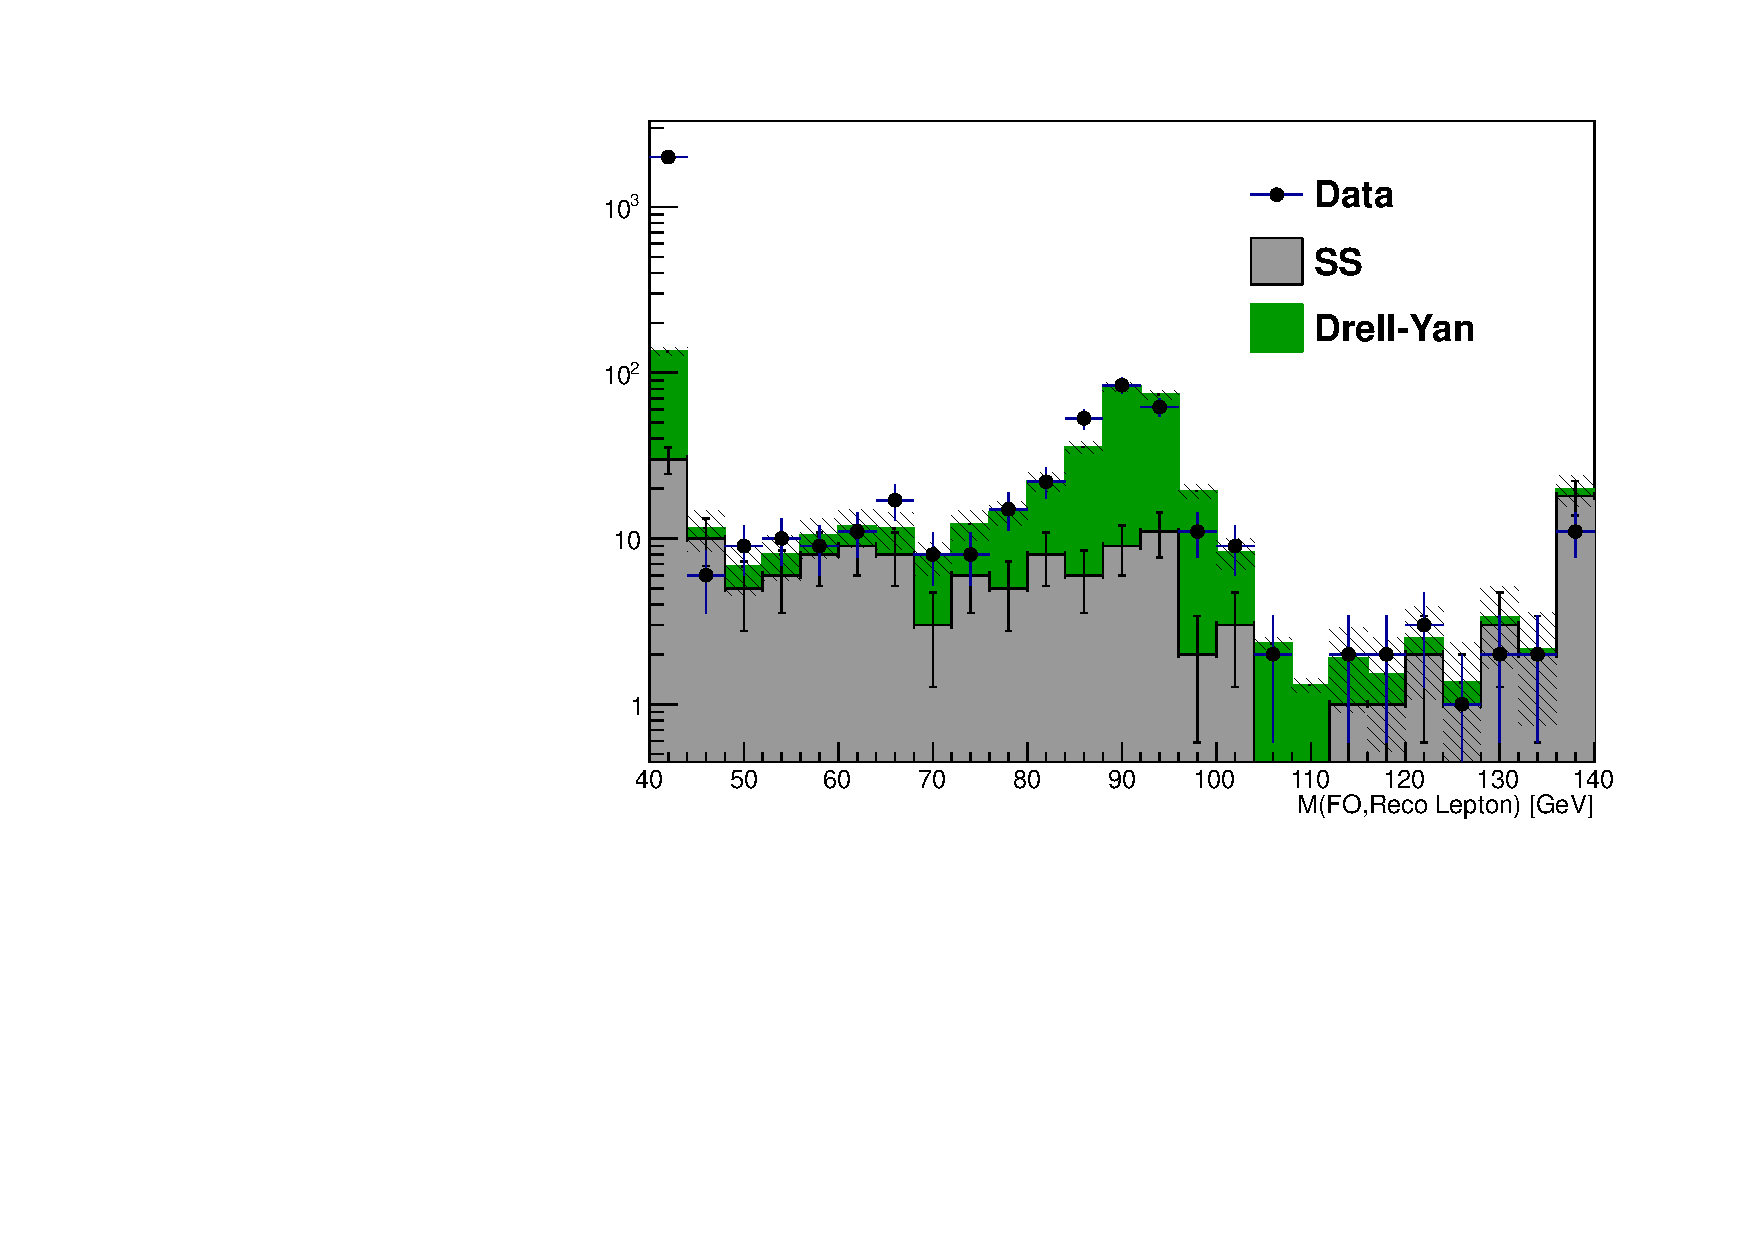
\includegraphics[width=.4\textwidth]{figures/ElectronFakeRate_V4_num_highPt_mll_met20mt15mll_Moriond_log.pdf}
}
\subfigure[]{
\centering
\label{subfig:mu_zjets_ctl}
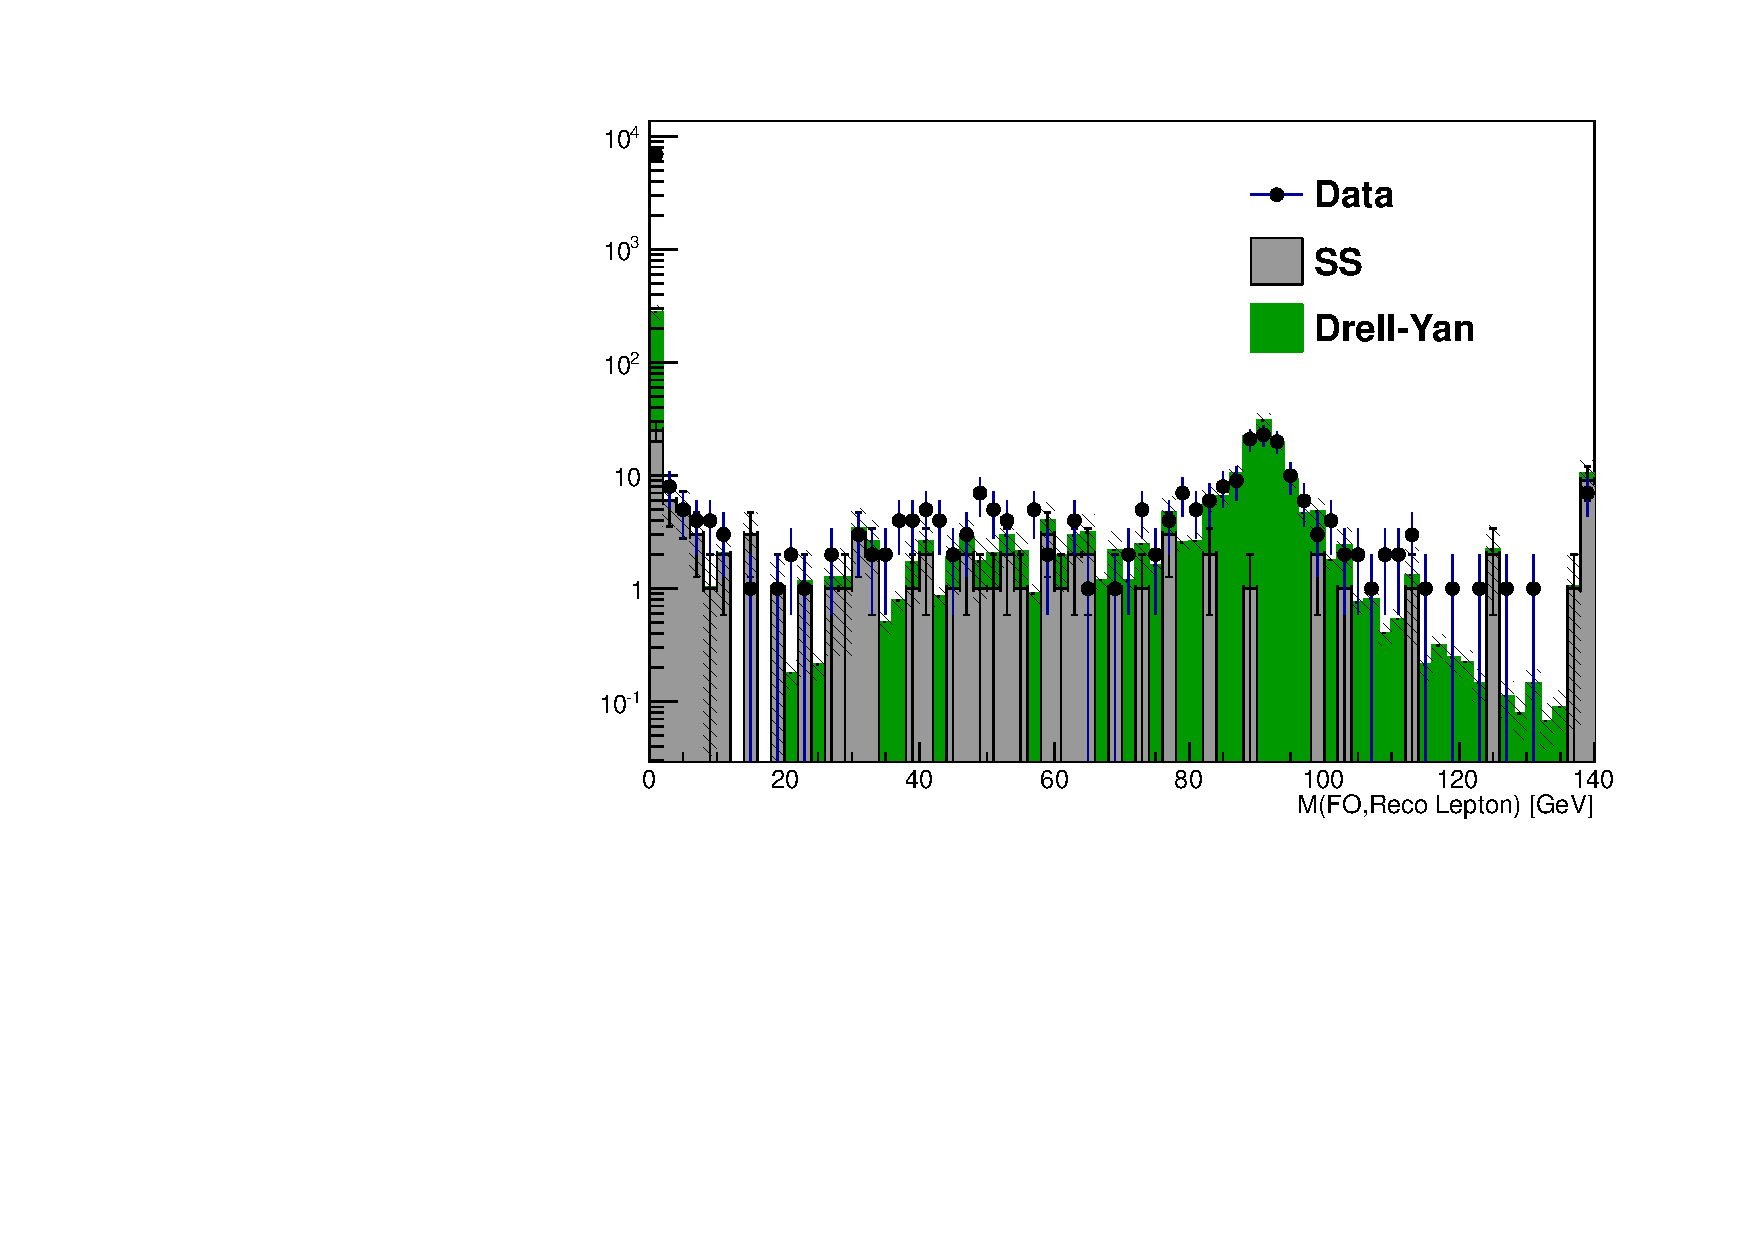
\includegraphics[width=.4\textwidth]{figures/MuonFakeRate_M2_num_highPt_mll_met20mt15mll_Moriond_log.pdf}
}\\
\caption{Z+Jets control region for muons (\ref{subfig:mu_zjets_ctl}) and electrons (\ref{subfig:el_zjets_ctl})
where FO passes the numerator and MET $<$ 20 GeV and MT $<$ 15 GeV and $76<\rm{Mll}<106$ GeV. 
The default jet pt threshold is applied, and the same sign yield is used to subtract the QCD background.}
\label{fig:zjets_ctl}
\end{figure}

To reject dielectron events where the second electron is 
outside of the tracker acceptance, we additionally require
the away jet to be within $|\eta|<2.5$. This requirement is 
not applied to the muon final state because a second muon
that falls out of the tracker acceptance will not be detected
by any other detector and thus the event will already 
fail the $\met$ veto. The distribution of the away jet $\eta$
is shown in Figure \ref{fig:awayjet_ctl}.

\begin{figure}[!hbtp]
\centering
\subfigure[]{
\centering
\label{subfig:el_awayjet_ctl}
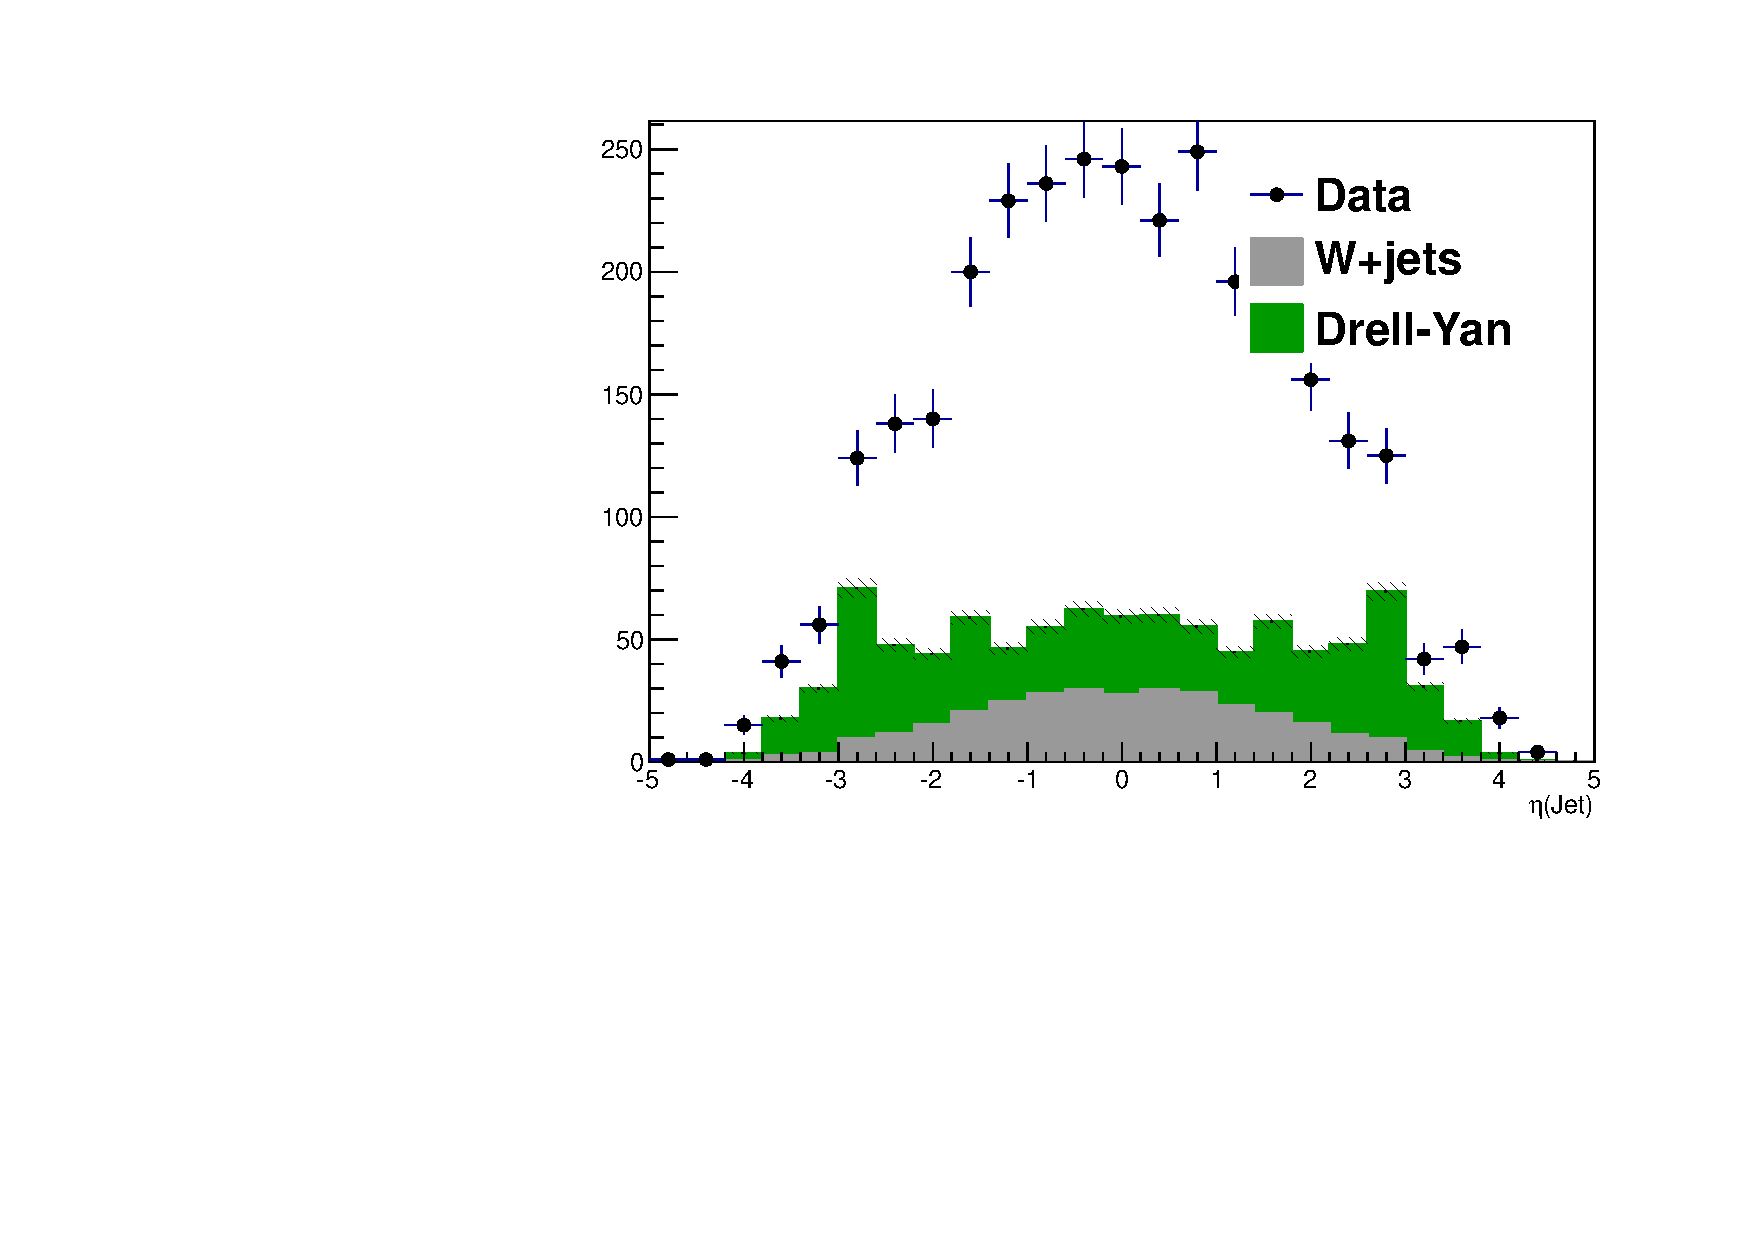
\includegraphics[width=.4\textwidth]{figures/ElectronFakeRate_V4_num_highPt_etaj_met20mt15mll_Moriond.pdf}
}
\subfigure[]{
\centering
\label{subfig:mu_awayjet_ctl}
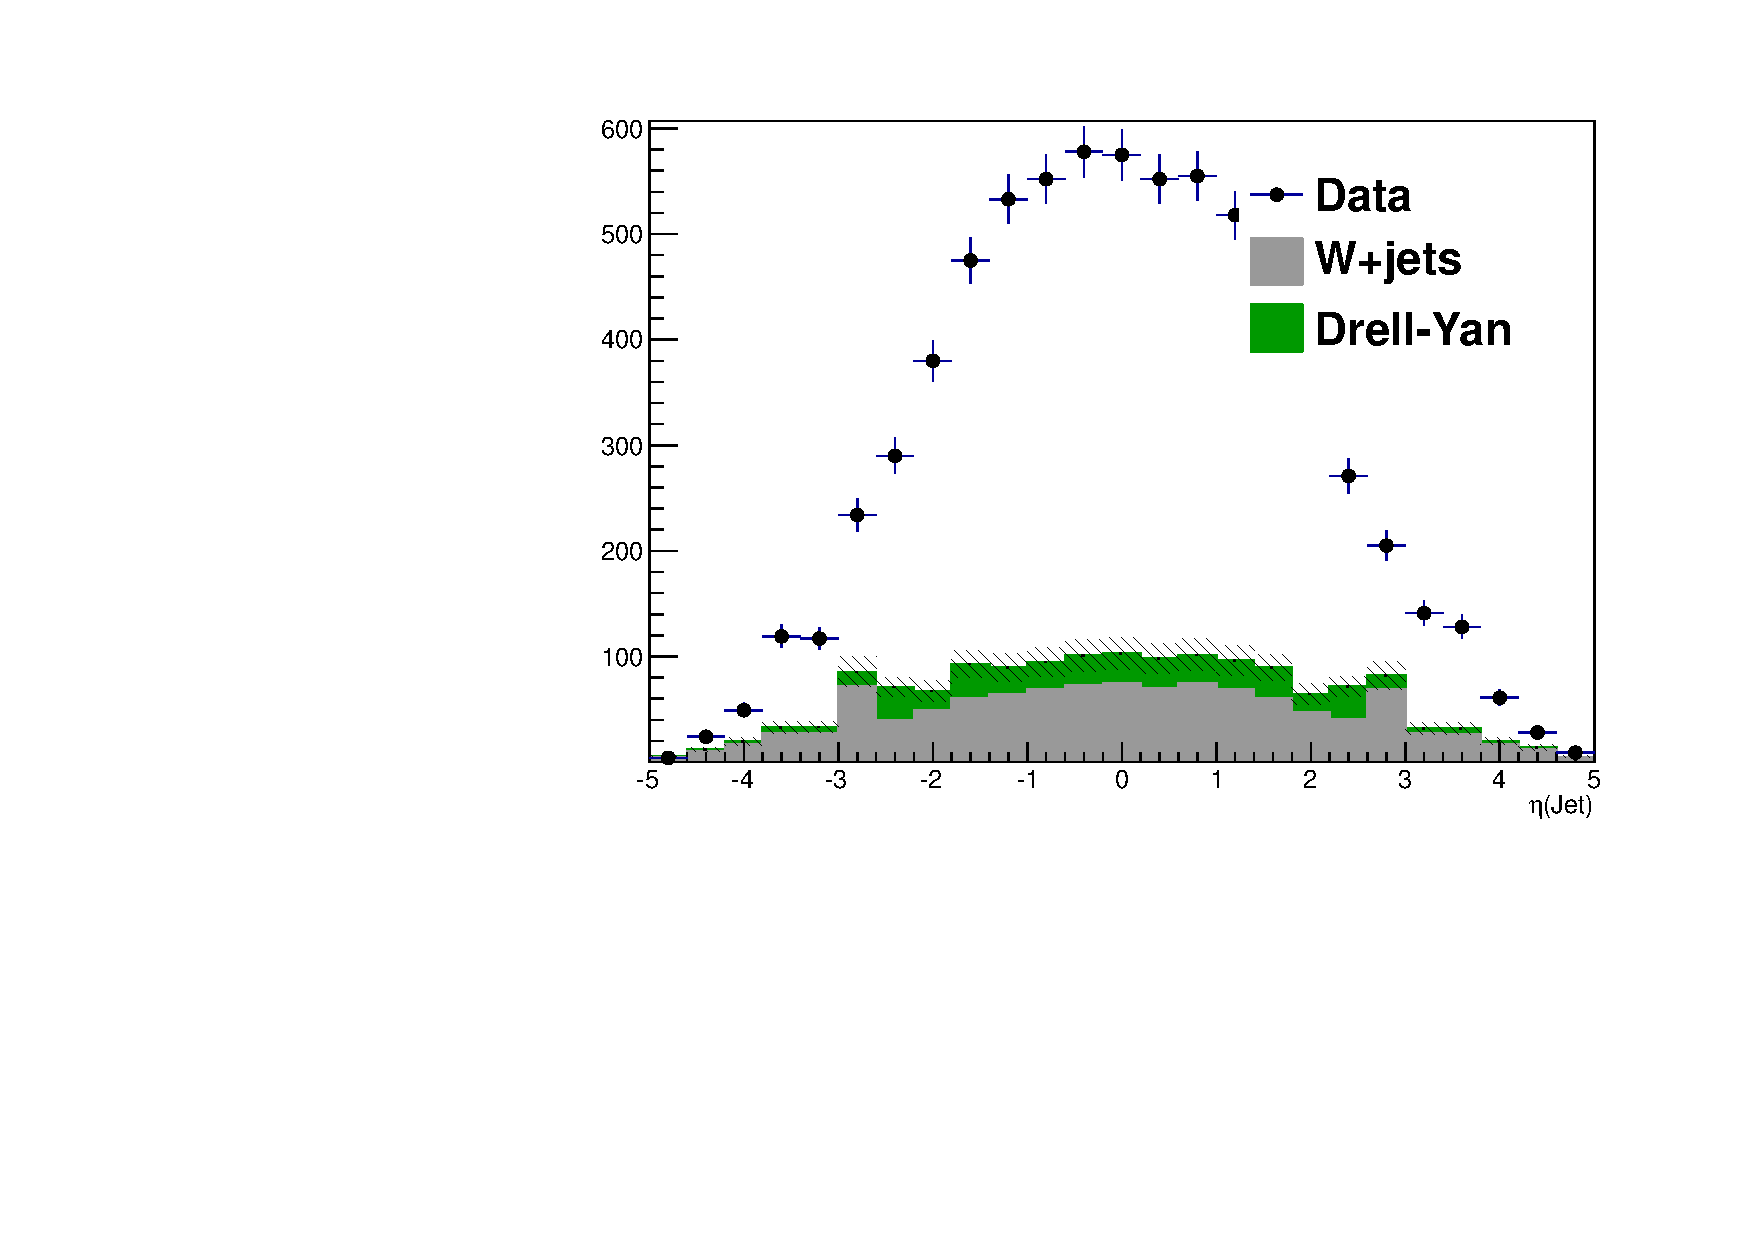
\includegraphics[width=.4\textwidth]{figures/MuonFakeRate_M2_num_highPt_etaj_met20mt15mll_Moriond.pdf}
}\\
\caption{Distribution of the leading away jet $\eta$ for muons (\ref{subfig:mu_awayjet_ctl}) and electrons (\ref{subfig:el_awayjet_ctl}). 
When deriving the electron fake rate, the region where the jet is beyond 2.5 is vetoed.}
\label{fig:awayjet_ctl}
\end{figure}

The muon fake rates before and after 
the electroweak background subtraction are given in
Tables \ref{tab:mufake_raw} and \ref{tab_mufake_cor} respectively.
The electron fake rates before and after          
the electroweak background subtraction are given in
Tables \ref{tab:elfake_raw} and \ref{tab_elfake_cor} respectively.
After applying the additional background reduction
requirements, the residual subtraction affects the fake rate
by up to 20\% in the electron case and up to 30\% in the muon case.
The change in the fake rate ompared to the HCP analysis \cite{hcp2012Note},
is up to 60\% at high $\pt$.  The total effect on the W+jets background
prediction is smaller than this because the cross-section for high $\pt$
fakes is smaller than at lower $\pt$.

%
% muons
%

\begin{table}[!ht]
{\small
\begin{center}
\begin{tabular}{c|c|c|c|c}
\hline
bin &  0.00 - 1.00  &   1.00 - 1.48  &   1.48 - 2.00  &   2.00 - 2.50 \\
\hline
  10.0 - 15.0  &    0.147 $\pm$ 0.002 &     0.166 $\pm$ 0.004 &     0.218 $\pm$ 0.004 &     0.270 $\pm$ 0.007 \\
  15.0 - 20.0  &    0.141 $\pm$ 0.006 &     0.169 $\pm$ 0.009 &     0.206 $\pm$ 0.011 &     0.262 $\pm$ 0.018 \\
  20.0 - 25.0  &    0.198 $\pm$ 0.004 &     0.232 $\pm$ 0.007 &     0.217 $\pm$ 0.007 &     0.257 $\pm$ 0.012 \\
  25.0 - 30.0  &    0.221 $\pm$ 0.008 &     0.257 $\pm$ 0.014 &     0.238 $\pm$ 0.014 &     0.293 $\pm$ 0.025 \\
  30.0 - 35.0  &    0.252 $\pm$ 0.015 &     0.313 $\pm$ 0.026 &     0.305 $\pm$ 0.026 &     0.349 $\pm$ 0.045 \\
\hline
\end{tabular}
\caption{Muon fake rate before background subtraction for jet pT $>$ 15}
\label{tab:mufake_raw}
\end{center}}
\end{table}
\begin{table}[!ht]
{\small
\begin{center}
\begin{tabular}{c|c|c|c|c}
\hline
bin &  0.00 - 1.00  &   1.00 - 1.48  &   1.48 - 2.00  &   2.00 - 2.50 \\
\hline
  10.0 - 15.0  &    0.146 $\pm$ 0.002 &     0.165 $\pm$ 0.004 &     0.217 $\pm$ 0.004 &     0.269 $\pm$ 0.007 \\
  15.0 - 20.0  &    0.137 $\pm$ 0.006 &     0.164 $\pm$ 0.009 &     0.202 $\pm$ 0.011 &     0.257 $\pm$ 0.018 \\
  20.0 - 25.0  &    0.184 $\pm$ 0.005 &     0.218 $\pm$ 0.008 &     0.200 $\pm$ 0.008 &     0.235 $\pm$ 0.013 \\
  25.0 - 30.0  &    0.187 $\pm$ 0.011 &     0.223 $\pm$ 0.016 &     0.199 $\pm$ 0.017 &     0.231 $\pm$ 0.030 \\
  30.0 - 35.0  &    0.187 $\pm$ 0.021 &     0.250 $\pm$ 0.031 &     0.236 $\pm$ 0.033 &     0.247 $\pm$ 0.057 \\
\hline
\end{tabular}
\caption{Muon fake rate after background subtraction for jet pT $>$ 15}
\label{tab:mufake_cor}
\end{center}}
\end{table}

%
% electrons
%

\begin{table}[!ht]
{\small
\begin{center}
\begin{tabular}{c|c|c|c|c}
\hline
bin &  0.00 - 1.00  &   1.00 - 1.48  &   1.48 - 2.00  &   2.00 - 2.50 \\
\hline
  10.0 - 15.0  &    0.068 $\pm$ 0.006 &     0.064 $\pm$ 0.007 &     0.024 $\pm$ 0.004 &     0.023 $\pm$ 0.005 \\
  15.0 - 20.0  &    0.074 $\pm$ 0.008 &     0.080 $\pm$ 0.010 &     0.026 $\pm$ 0.005 &     0.032 $\pm$ 0.006 \\
  20.0 - 25.0  &    0.070 $\pm$ 0.004 &     0.096 $\pm$ 0.006 &     0.038 $\pm$ 0.004 &     0.045 $\pm$ 0.004 \\
  25.0 - 30.0  &    0.080 $\pm$ 0.006 &     0.101 $\pm$ 0.008 &     0.044 $\pm$ 0.005 &     0.043 $\pm$ 0.005 \\
  30.0 - 35.0  &    0.090 $\pm$ 0.007 &     0.115 $\pm$ 0.010 &     0.049 $\pm$ 0.006 &     0.062 $\pm$ 0.007 \\
\hline
\end{tabular}
\caption{Electron fake rate before background subtraction for jet pT $>$ 35}
\label{tab:elfake_raw}
\end{center}}
\end{table}
\begin{table}[!ht]
{\small
\begin{center}
\begin{tabular}{c|c|c|c|c}
\hline
bin &  0.00 - 1.00  &   1.00 - 1.48  &   1.48 - 2.00  &   2.00 - 2.50 \\
\hline
  10.0 - 15.0  &    0.067 $\pm$ 0.006 &     0.063 $\pm$ 0.007 &     0.023 $\pm$ 0.004 &     0.023 $\pm$ 0.005 \\
  15.0 - 20.0  &    0.071 $\pm$ 0.008 &     0.077 $\pm$ 0.010 &     0.025 $\pm$ 0.005 &     0.031 $\pm$ 0.006 \\
  20.0 - 25.0  &    0.063 $\pm$ 0.004 &     0.091 $\pm$ 0.006 &     0.036 $\pm$ 0.004 &     0.043 $\pm$ 0.004 \\
  25.0 - 30.0  &    0.068 $\pm$ 0.006 &     0.093 $\pm$ 0.008 &     0.039 $\pm$ 0.005 &     0.041 $\pm$ 0.005 \\
  30.0 - 35.0  &    0.070 $\pm$ 0.008 &     0.102 $\pm$ 0.011 &     0.043 $\pm$ 0.006 &     0.058 $\pm$ 0.007 \\
\hline
\end{tabular}
\caption{Electron fake rate after background subtraction for jet pT $>$ 35}
\label{tab:elfake_cor}
\end{center}}
\end{table}

